\section{System's perspective} \label{section:System perspective}
\todo{argue for the choice of technologies and decisions for at least all cases for which we asked you to do so in the tasks at the end of each session.}
\subsection{Design} %Jonas
\hyperref[fig:componentDiagram]{Figure \ref{fig:componentDiagram}} shows the different components of the ITU-minitwit system.

\todo{TODO: MISSING TEXT ON EACH CONNECTOR.}
\begin{figure}[H]
    \centering
    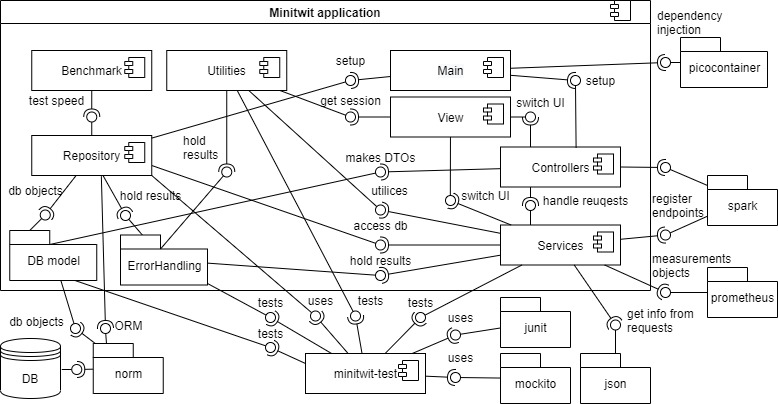
\includegraphics[width=1.0\textwidth]{images/Diagrams-Development_view_component_diagram.jpg}
    \caption{Component diagram, development view}
    \label{fig:componentDiagram}
\end{figure}


\begin{itemize}
    \item \textbf{Main}: is the entrance point onto the program, and contains arguments to modify which database is used. Main also starts the maintenance and defines the max number of threads for the program.\\
    The class diagram can be seen in \hyperref[fig:classDiagramMain]{figure \ref{fig:classDiagramMain}}.
    \begin{figure}[H]
        \centering
        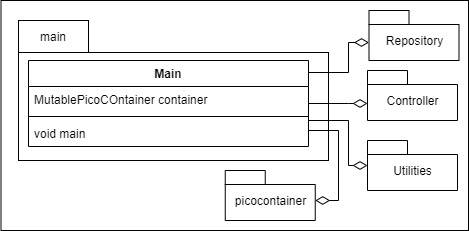
\includegraphics[width=1.0\textwidth]{images/class_diagram_main.jpg}
        \caption{Class diagram main, logical view}
        \label{fig:classDiagramMain}
    \end{figure}
    
    \item \textbf{Utilities}: contains helper methods like hashing, formatting dates and JSON, as well as housing Request, Response and Session wrapper objects. \\
    The class diagram can be seen in \hyperref[fig:classDiagramUtilities]{figure \ref{fig:classDiagramUtilities}}.
    \begin{figure}[H]
        \centering
        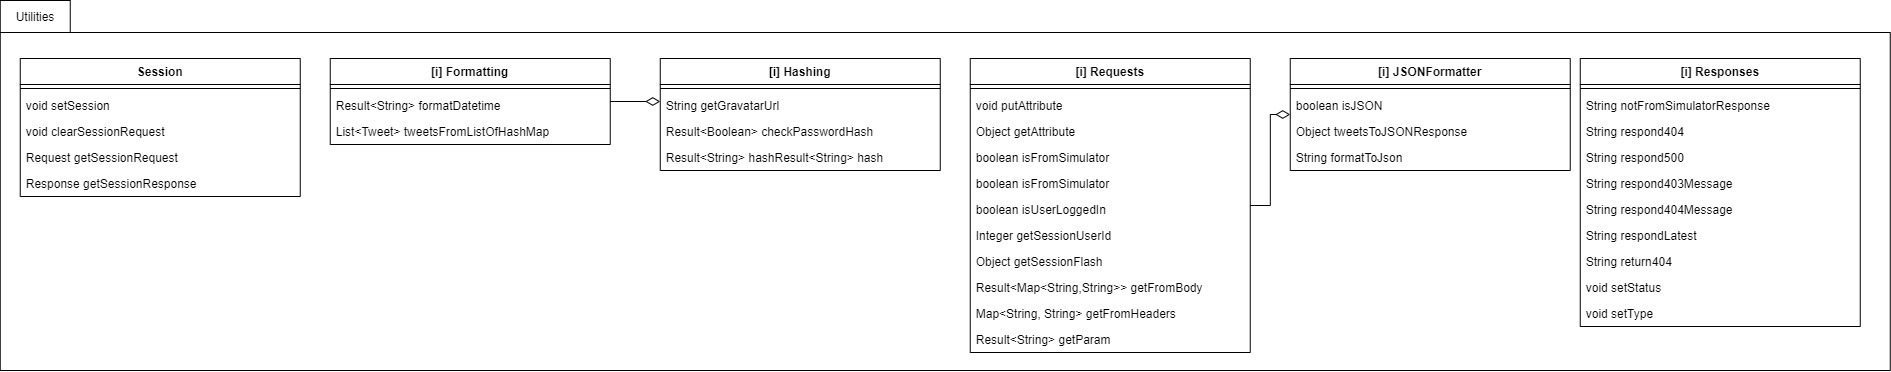
\includegraphics[width=1.0\textwidth]{images/class_diagram_utilities.jpg}
        \caption{Class diagram utilities, logical view}
        \label{fig:classDiagramUtilities}
    \end{figure}
    
    \item \textbf{Error handling}: Contains objects to hold result of computations which could result in exceptions, allowing for better error handling and reducing amounts of try-catch statements. \\
    The class diagram can be seen in \hyperref[fig:classDiagramErrorhandling]{figure \ref{fig:classDiagramErrorhandling}}.
    \begin{figure}[H]
        \centering
        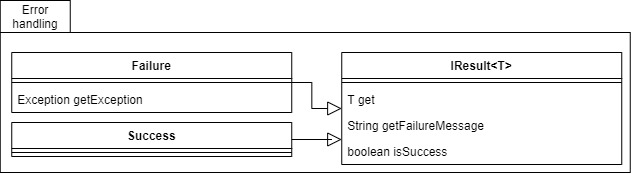
\includegraphics[width=1.0\textwidth]{images/class_diagram_errorhandling.jpg}
        \caption{Class diagram errorhandling, logical view}
        \label{fig:classDiagramErrorhandling}
    \end{figure}
    
    \item \textbf{Controllers}: Handles the different endpoints which our website should provide, by mapping paths for post and get request to which code should handle the requests and responses.\\
    The class diagram can be seen in \hyperref[fig:classDiagramControllers]{figure \ref{fig:classDiagramControllers}}.
    \begin{figure}[H]
        \centering
        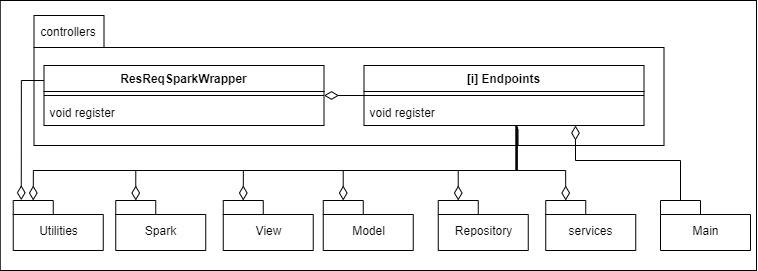
\includegraphics[width=1.0\textwidth]{images/class_diagram_controllers.jpg}
        \caption{Class diagram controllers, logical view}
        \label{fig:classDiagramControllers}
    \end{figure}
    
    \item \textbf{View}: Contains code for changing what is presented in the website, by redirecting to new paths or by setting new HTML file/template to be used along with variables for it to know.\\
    The class diagram can be seen in \hyperref[fig:classDiagramView]{figure \ref{fig:classDiagramView}}.
    \begin{figure}[H]
        \centering
        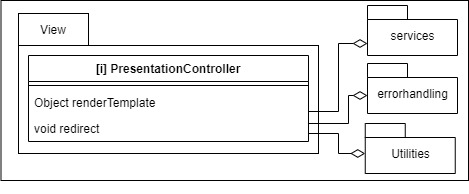
\includegraphics[width=1.0\textwidth]{images/class_diagram_view.jpg}
        \caption{Class diagram view, logical view}
        \label{fig:classDiagramView}
    \end{figure}
    
    \item \textbf{Services}: Includes the code for maintenance, which uses Prometheus library to store the values Prometheus should collect, and the log service, which prints in a manner easy to filer for in Kibana. Services also includes functions executing the requests and responses.\\
    The class diagram can be seen in \hyperref[fig:classDiagramServices]{figure \ref{fig:classDiagramServices}}.
    \item \textbf{Repository}: Includes code for starting the database and for executing queries needed by the services. 
    
    The ORM tool used is \textit{NORM}, which is a lightweight ORM that does not require the complex markdown files that \textit{Hibernate}, \textit{JPA} etc. introduce. It is suitable for smaller projects with simple models and therefore for the Minitwit application. Another ORM tool, \textit{Hibernate}, was tried in order to see if it would be a better fit than NORM since it is more complex but it turned out that the tool did not deliver on its promises, meaning that it only introduced more unnecessary complexity without adding any benefits. It furthermore complicated database joins that are needed in the Minitwit application. It was therefore decided to stick with \textit{NORM}. The class diagram can be seen in \hyperref[fig:classDiagramRepository]{figure \ref{fig:classDiagramRepository}}.
    \begin{figure}[H]
        \centering
        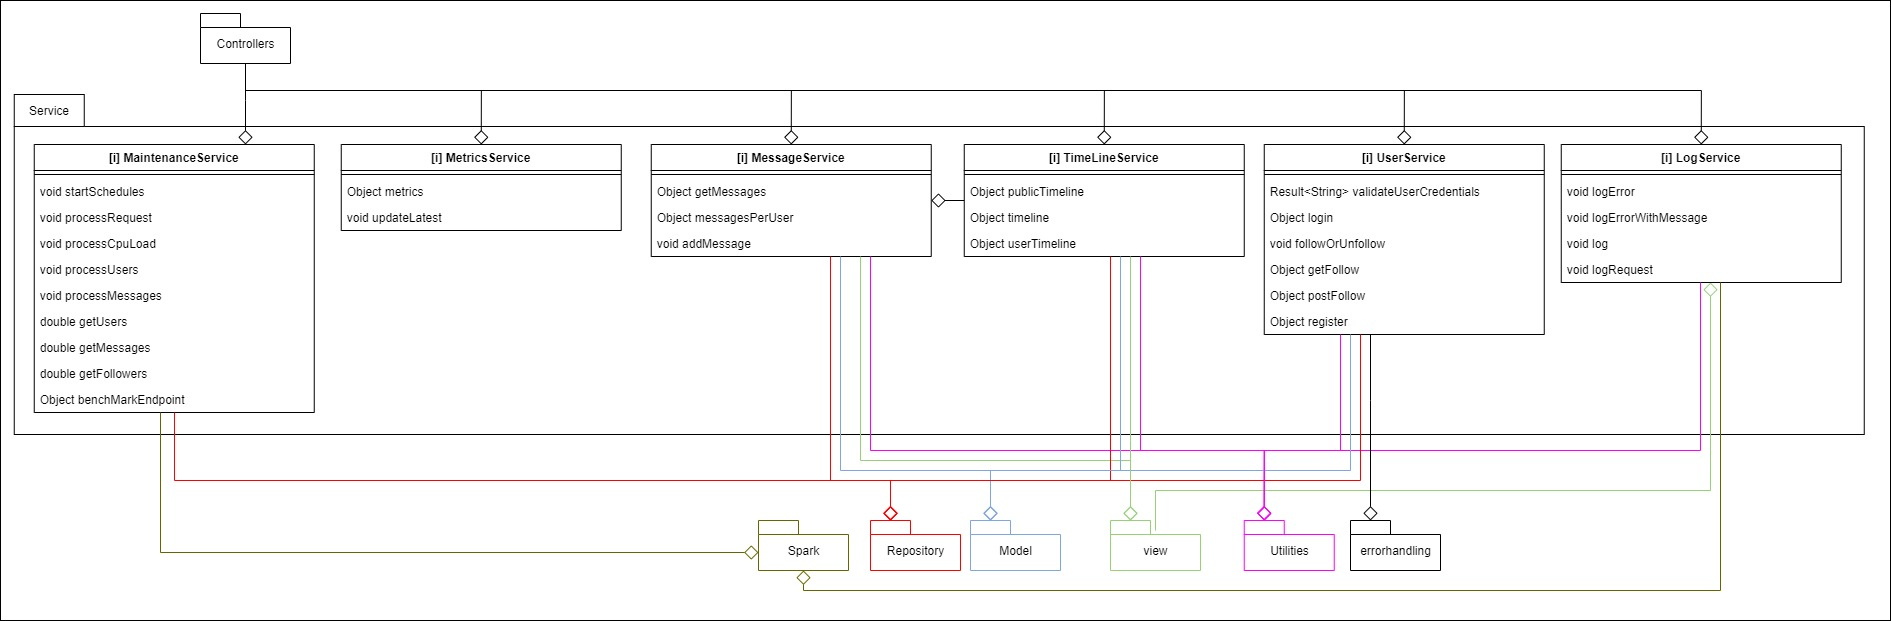
\includegraphics[width=1.0\textwidth]{images/class_diagram_services.jpg}
        \caption{Class diagram services, logical view}
        \label{fig:classDiagramServices}
    \end{figure}
    
    \item \textbf{Model}: Model contains the database relations with one object per entity. The objects in the folder matches the entities in the database as they are the template NORM uses to create it.\\
    The class diagram can be seen in \hyperref[fig:classDiagramModel]{figure \ref{fig:classDiagramModel}}.
    \begin{figure}[H]
        \centering
        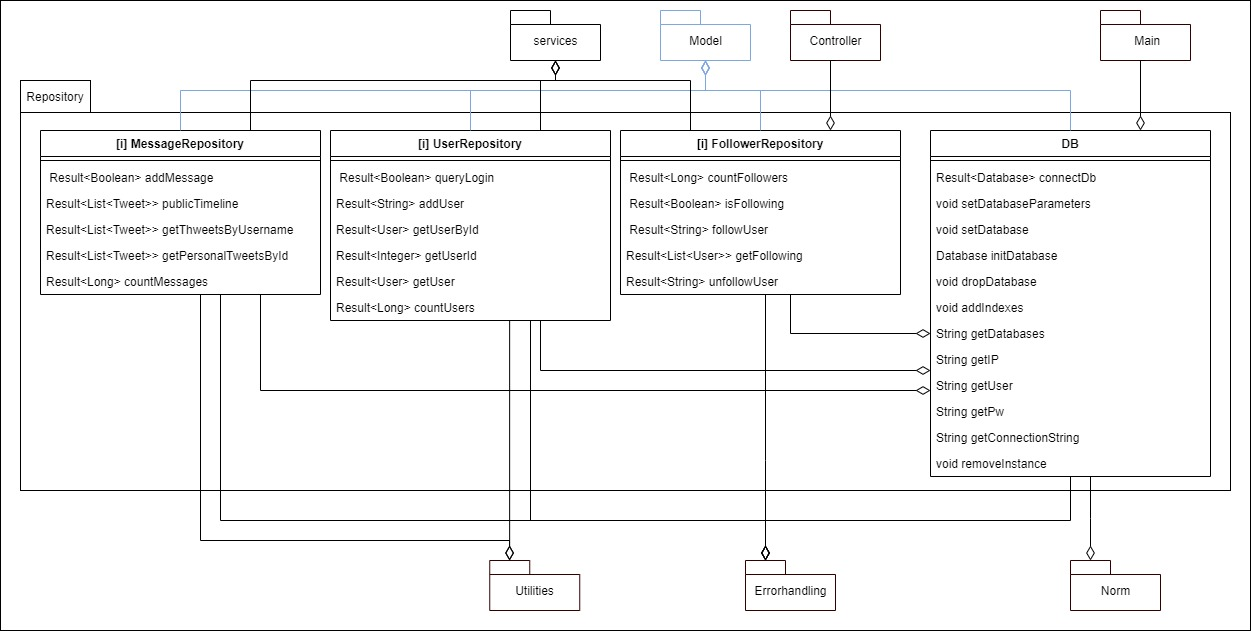
\includegraphics[width=1.0\textwidth]{images/class_diagram_repository.jpg}
        \caption{Class diagram repository, logical view}
        \label{fig:classDiagramRepository}
    \end{figure}

    \item \textbf{Benchmark}: This is not in deployment and contains code to be run locally only. The packet component relates to measuring speed of different operations in the repository and was used to argue for speedups related to any extension to a database of same size as the one in deployment, as when indexes was added.\\
    The class diagram can be seen in \hyperref[fig:classDiagramModel]{figure \ref{fig:classDiagramModel}}.
    \begin{figure}[H]
        \centering
        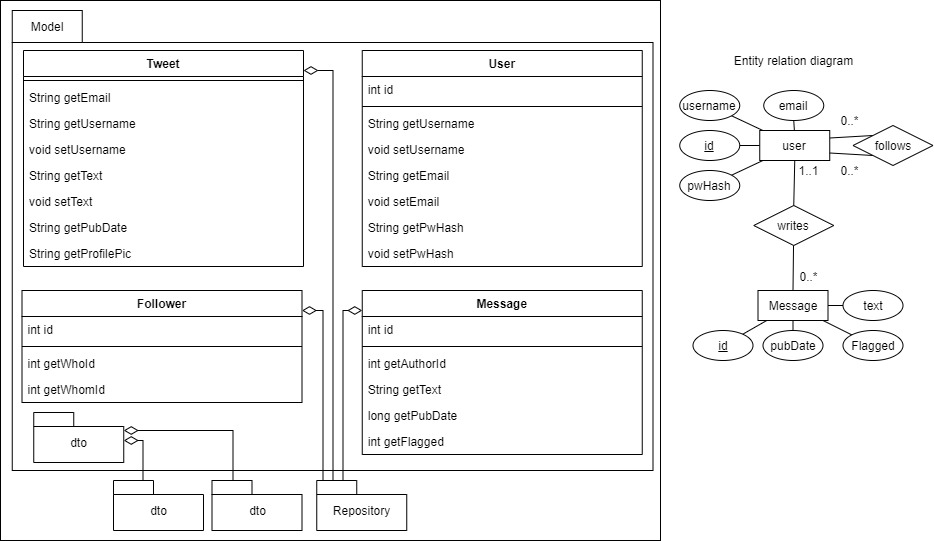
\includegraphics[width=1.0\textwidth]{images/class_diagram_model.jpg}
        \caption{Class diagram model, logical view}
        \label{fig:classDiagramModel}
    \end{figure}
\end{itemize}


\subsection{Architecture} %Jonas
\hyperref[fig:componentDiagram]{Figure \ref{fig:componentDiagram}} shows the architecture of the entire ITU-minitwit system.\\
Code is stored in Github, which developers pull and push to during development. As mentioned main contains code for which database to use, and when running just the code locally it should use a local database called minitwit running on port 3306 localhost with password and username "root". When running locally with docker compose the MySQL services should be stopped so a container for the database can be created.\\
Github actions test the files pushes using sonar cloud. Github actions also deploy to a docker image and pull down official Prometheus, Grafana, Filebeat, ElasticSearch, Kibana and Nginx images.\\
The images are deployed on a digital ocean server containing one database and 2 digital ocean droplets. Each droplet contain a minitwit application and an official image. One image's floating point IP is in production and the other use heartbeat test whether primary is still up or whether it should become the new primary.
\todo{Heartbeat}\\
The Prometheus and Grafana images are for viewing maintenance and other four are for logging purposes.




\begin{figure}[H]
    \centering
    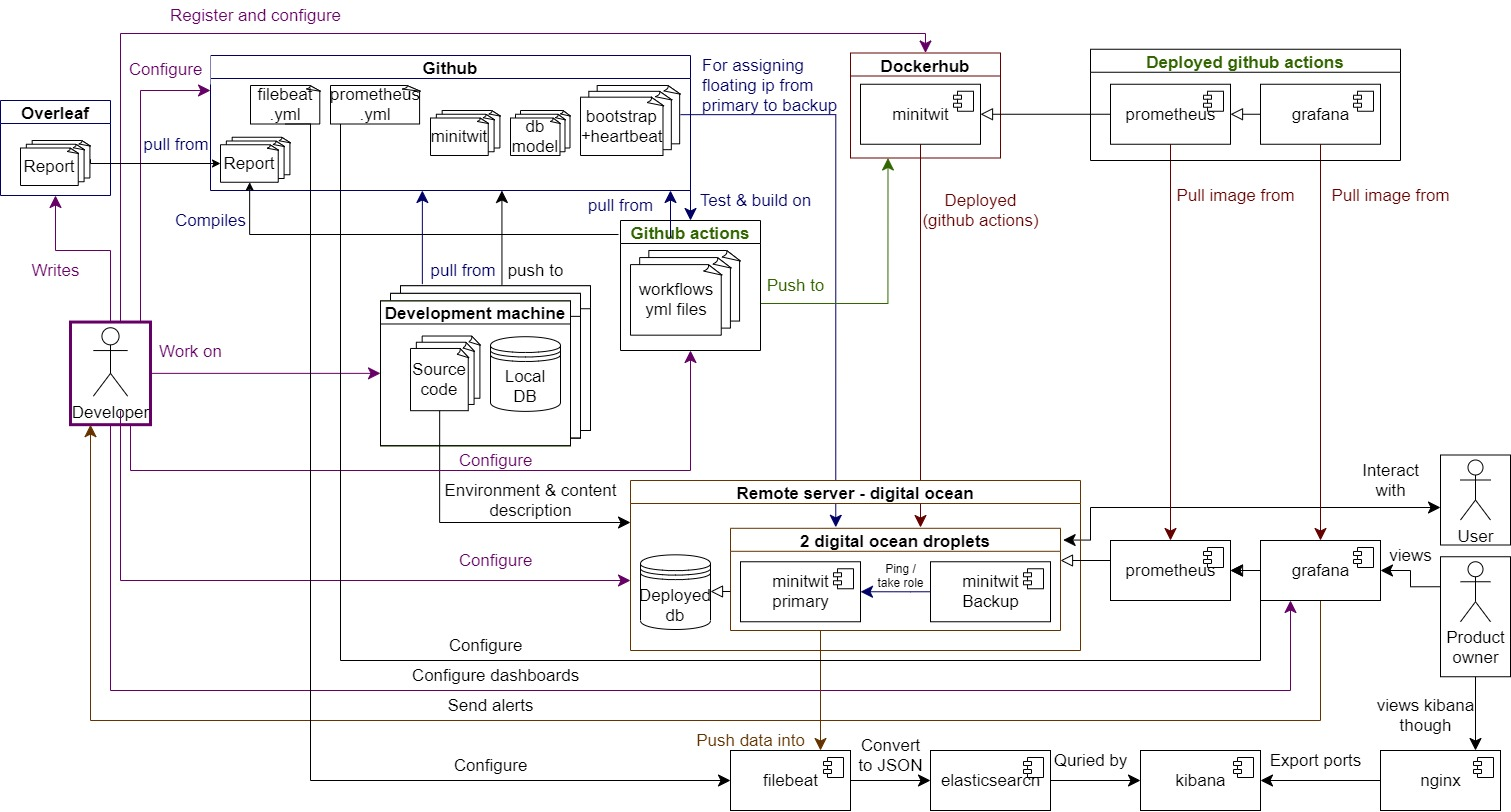
\includegraphics[width=1.0\textwidth]{images/Diagrams-Process_view_communication_diagram.jpg}
    \caption{Communication diagram, process view}
    \label{fig:componentDiagram}
\end{figure}





\subsection{Dependencies } %Nikolaj %god ide med license her
\begin{itemize}
    \item \textbf{Spark Java}:A micro framework for creating web applications with minimal effort. Suitable for the minitwit project size and gave us the freedom to structure the application how we wanted it.
    \item \textbf{jinjava}: template engine based on django template syntax, used to render jinja templates. Chosen to mimic the python minitwit with minimal effort. 
    \item \textbf{PicoContainer}: General purpose IoC container.
    \item \textbf{NORM}: Lightweight ORM that doesn't require the complex markdown files that Hibernate, JPA etc. introduce. Suitable for smaller projects with simple models. 
    \item \textbf{MySQL}: Relational database. Chosen based on familiarity to team members and it's renowned reliability for how long it's been around.  
    \item \textbf{JUnit 5}: Most popular unit-testing framework.
    \item \textbf{Mockito}: Mocking framework with a simple API.
    \item \textbf{SLF4J}: Logging Facade for ELK stack. 
    \item \textbf{prometheus}: Prometheus JVM Client for introducing instrumenting such as gauges, counters and other metrics.
    \item \textbf{org.json}: Toolkit for JSON.
\end{itemize}
\subsubsection{Plugins}
\begin{itemize}
    \item \textbf{Maven}: Build automation tool used to manage our Java project and its dependencies.
    \item \textbf{PMD}: code analyzer, used to find common programming flaws like unused variables, unnecessary object creation etc. 
    \item \textbf{Forbidden API Checker}: Static code analysis that parses java byte code to find invocations of dangerous and deprecated method/class/fields signatures. 
    \item \textbf{SonarCloud}: Bug, Vulnerability and Code Smell detection with issue contextualization and remediation guidance. Used in our CI for Continuous code inspection.
\end{itemize}
\footnote{\url{https://github.com/DevOps2021-gb/devops2021/wiki/Static-Analysis-Tools}}

\todo{Skal plugins nævnes?(maven, PMD, forbiddenAPIs) \textcolor{yellow}{Maven kunne måske være relevant i hvert fald}}


We used \url{www.licensediscovery.io} to analyze our Maven dependency licenses. As seen in figure \ref{fig:licenceDep} the strictest license that the majority of dependencies is ruled by is the Apache Software License Version 2. This is the license that we therefore went with.\footnote{\url{https://github.com/DevOps2021-gb/devops2021/blob/main/LICENSE.md}} \todo{Er det begrundelse nok?}
\begin{figure}[!htb]
    \centering
    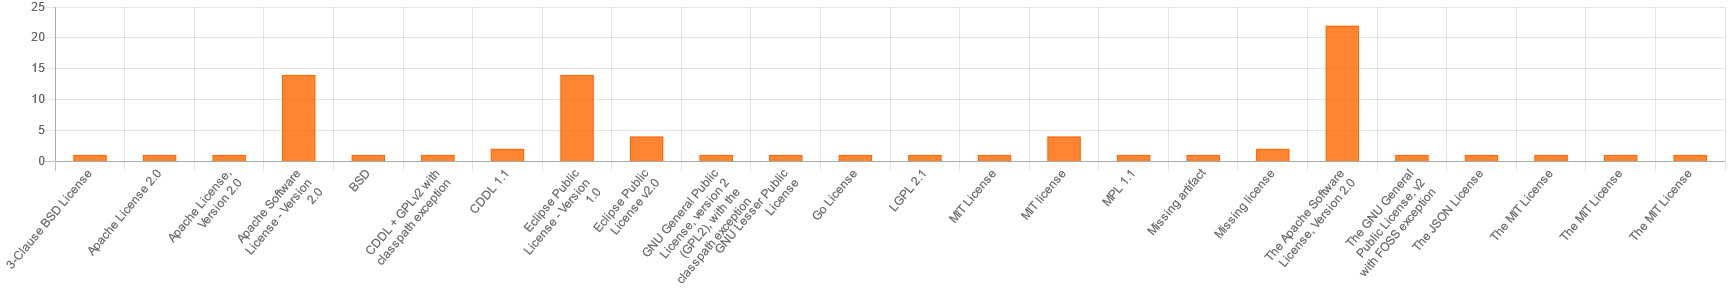
\includegraphics[scale=0.2]{images/LicenceDependencies.png}
    \caption{Overview of dependency licenses. Sub-dependencies included.}
    \label{fig:licenceDep}
\end{figure}


\subsection{Important interactions of subsystem}

\subsection{Current state of system}
The system is currently has a single known bug regarding the scaling of the system, see section \ref{issues-operation}. The tool used for static analysis, \texttt{Sonarcloud}, reports the best rating, \textit{A}, on all measures, with 

\begin{itemize}
    \item 0 bugs
    \item 0 code vulnerabilities and 0 security hotspots
    \item 6 hours code debt due to 63 code smells
    \item 0.0\% code duplication and 0 duplicated blocks
\end{itemize}

Out of the 63 code smells only 11 are major, critical or blockers and all 63 has been assessed as issues that can ignored.

